\documentclass{article}
\usepackage[spanish]{babel}
\usepackage[utf8]{inputenc}
\usepackage{amsmath}
\usepackage{graphicx}
\graphicspath{ {images/} }
\usepackage{xcolor}
\usepackage{listings}
\lstset{
	language=java,
	numberstyle=\tiny, 
	breaklines=true,
	numbersep=1pt,
	tabsize=2,
	postbreak=\raisebox{0ex}[0ex][0ex]{\ensuremath{\color{red}\hookrightarrow\space}},
	numbers=left
}
\usepackage{floatflt}
\usepackage{multicol}
\usepackage{geometry}
\geometry{landscape,letterpaper,tmargin=1cm,bmargin=2cm,lmargin=1cm,rmargin=1cm}
\setlength{\columnsep}{0.25in}
\setlength{\columnseprule}{1px}


\begin{document}

\begin{multicols}{2}

\tableofcontents

\section{Notas previas - IMPORTANTE LEER}
\begin{itemize}
	\item Se usarán algunas clases estándar de Java para simplificar las cosas
	\item No se presenta el código implementado de todas las fórmulas, ya que muchas pueden ser programadas fácilmente
	\item \( \pi \) está definido en Java en la constante Math.PI
	\item Se trabajará siempre con los ángulos en {\bf radianes}. Para convertir un ángulo \( \alpha \) en grados, en uno en radianes \( \theta \): \( \theta = (\alpha \cdot \pi) / 180 \)
	\item  El enunciado de los problemas generalmente establece un margen de error. Ese es el épsilon que se usará para las comparaciones entre números de punto flotante. Usualmente lo defino como variable estática de clase (por ejmplo, \emph{static double eps = 1e-6;}).
\end{itemize}


\section{Puntos}
Para representar un punto se usa la clase de Java \emph{Point2D.Double}
\lstinputlisting[firstline=6, lastline=7]{./src/Puntos.java}

\subsection{Distancia entre dos puntos}
\[ d = \sqrt{(x_2-x_1)^{2} + (y_2-y_1)^{2}} \]

Se puede usar un método de Java:
\lstinputlisting[firstline=9, lastline=9]{./src/Puntos.java}

También hay un método que devuelve el cuadrado de la distancia, para evitar sacar la raíz cuadrada y perder precisión:
\lstinputlisting[firstline=10, lastline=10]{./src/Puntos.java}

\subsection{Rotar un punto}
Se rota un punto \( (x, y) \) por un ángulo \( \theta \) en sentido {\bf antihorario}.
\lstinputlisting[firstline=13, lastline=17]{./src/Puntos.java}

\section{Vectores}
Sean dos puntos \( p_1 = (x_1, y_1) \) y \( p_2 = (x_2, y_2) \). El vector que va desde \( p_1 \) hacia \( p_2 \) se define como:
\[ V = \langle v_1, v_2 \rangle \ = \langle x_2 - x_1, \, y_2 - y_1 \rangle \]

Sugiero representarlos con un array de tipo \emph{double} (\emph{double[] v}).

\subsection{Magnitud de un vector}
\[ |V| = \sqrt{v_1^2 + v_2^2} \]

\subsection{Dirección de un vector}
El ángulo entre un vector \( V = \langle v_1, v_2 \rangle \ \) y los ejes \( x \) y \( y \) es:
\[ \cos \theta_x = \frac{v_1}{|V|}, \quad \cos \theta_y = \frac{v_2}{|V|} \]

En Java la función para sacar el coseno inverso (y poder despejar \( \theta \) en estas fórmulas) es \emph{Math.acos}

\subsection{Vectores paralelos y perpendiculares}
\lstinputlisting[firstline=37, lastline=45]{./src/Lineas.java}

\subsection{Ángulo entre vectores}
El menor ángulo entre dos vectores \( A = \langle a_1, a_2 \rangle \) y \( B = \langle b_1, b_2 \rangle \) es:
\[ \cos \theta = \frac{a_1 b_1 + a_2 b_2}{|A| |B|} \]

En Java la función para sacar el coseno inverso (y poder despejar \( \theta \) en esta fórmula) es \emph{Math.acos}


\section{Líneas}
Para representar una recta definida por dos puntos se usa la clase de Java \emph{Line2D.Double}
\lstinputlisting[firstline=9, lastline=11]{./src/Lineas.java}

\subsection{Distancias}

\subsubsection{Distancia de un punto a una recta}
\lstinputlisting[firstline=13, lastline=14]{./src/Lineas.java}

\subsubsection{Distancia de un punto a un segmento}
\lstinputlisting[firstline=16, lastline=19]{./src/Lineas.java}

\subsubsection{Distancia entre dos segmentos}
Sean dos segmentos \(s_1, s_2 \). La distancia más corta entre ellos es:
\lstinputlisting[firstline=22, lastline=35]{./src/Lineas.java}	 

\subsection{Verificar si dos rectas son paralelas o perpendiculares}
Se puede hacer utilizando vectores, pero con este método no se puede especificar el punto de intersección, o determinar si las dos rectas son la misma  (en caso de requerir esto, ver la siguiente sección, 4.3).

Usa la función de vectores paralelos y perpendiculares (ver sección 3.3).
\lstinputlisting[firstline=47, lastline=51]{./src/Lineas.java}

\subsection{Interseción de dos rectas}
Si las dos rectas no son paralelas, se intersectan en un punto. Se halla la ecuación general de ambas rectas y se soluciona un sistema lineal de ecuaciones para hallar el punto de intersección.

La ecuación general de una recta tiene la forma \( Ax+By+C=0 \).
\lstinputlisting[firstline=53, lastline=85]{./src/Lineas.java}

\subsection{Verificar si tres puntos son colineales}
Se puede usar, por ejmplo, para verificar si el punto \( p_3 \) pertenece a la recta definida por los puntos \( p_1 \) y \( p_2 \).
\lstinputlisting[firstline=87, lastline=95]{./src/Lineas.java}


\section{Círculos}
Un círculo se define con un centro \( (x_0, y_0) \) y un radio \( r \).

\subsection{Área y perímetro}
Área: \( \pi r^2 \)

Perímetro:  \( 2 \pi r \)

\subsection{Determinar si un punto está dentro o fuera de un círculo}
\lstinputlisting[firstline=7, lastline=17]{./src/Circulos.java}

\subsection{Arco, sector, cuerda y segmento}
% 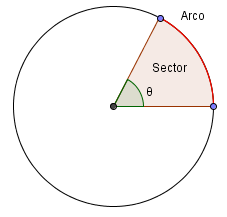
\includegraphics{sector}

Longitud del Arco: \( r \theta \)

Área del Sector: \( \frac{r^2 \theta}{2} \)

Longitud de la Cuerda: \( 2 r \cdot \sin (\frac{\theta}{2} ) \)

Área del Segmento: \( \frac{r^2}{2} \cdot ( \theta - \sin \theta ) \)

\subsection{Círculo formado por 3 puntos}
Sean tres puntos  \( p_1 \), \( p_2 \) y  \( p_3 \). Si no son colineales, existe un círculo que pasa por los tres. Se hallan los coeficientes de la ecuación general de la circunferencia \( x^2+y^2+Ax+By+C=0 \), de los cuales se puede extraer el radio y el centro de la misma.
\lstinputlisting[firstline=19, lastline=49]{./src/Circulos.java}

\subsection{Recta tangente a un círculo}
Es posible hallar la ecuación general de la recta tangente en un punto \( (x_1, y_1) \) a una circunferencia con centro \( (x_0, y_0) \) y radio \( r \). 

Sean \( w = x_1-x_0 \) y \( t = y_1-y_0 \). La ecuación general de la recta tangente es:
\[ wx + ty + (-wx_0 - ty_0 - r^2) = 0 \]

\section{Triángulos}

% 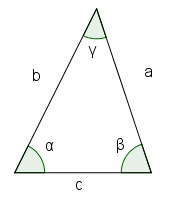
\includegraphics{triangulo}

\subsection{Desigualdad triangular}
Todo triángulo cumple las siguientes desigualdades:
\[ a+b > c \qquad a+c > b \qquad b+c>a \]

\subsection{Área de un triángulo dados sus lados}
Sea el \( s \) el semiperímetro del triángulo:
\[ s = \frac{a+b+c}{2} \]

El área del triángulo es (fórmula de Herón):
\[ A = \sqrt{s(s-a)(s-b)(s-c)} \]

\subsection{Área de un triángulo dados sus puntos}
Si se tienen las coordenadas \( (x_i, y_i) \) de los tres puntos que definen un triángulo, su área es:
\[ A = \frac{1}{2} \cdot | x_1(y_2-y_3) + x_2(y_3-y_1) + x_3(y_1-y_2) | \]

\subsection{Ley del seno y del coseno}
\[ \frac{a}{\sin(\alpha)} = \frac{b}{\sin(\beta)} = \frac{c}{\sin(\gamma)} \]

\[ a^2 = b^2 + c^2 - 2bc \cdot \cos(\alpha) \]
\[ b^2 = a^2 + c^2 - 2ac \cdot \cos(\beta) \]
\[ c^2 = a^2 + b^2 - 2ab \cdot \cos(\gamma) \]

\subsection{Círculo inscrito y circunscrito}
\[ r_i = \frac{A}{s}, \quad r_c = \frac{abc}{4A} \]


\section{Polígonos}
Un polígono de \( n \) puntos se representa como un vector de \( n \) posiciones de tipo \emph{Point2D.Double}.

Se asume por defecto que los puntos {\bf están ordenados en sentido antihorario}. Si el polígono no está ordenado, estos algoritmos no sirven. Habría que ordenarlo primero.

\subsection{Perímetro}
\lstinputlisting[firstline=9, lastline=17]{./src/Poligonos.java}

\subsection{Área}
El algoritmo sólo sirve para polígonos simples (que no se intersectan a sí mismos). Si el polígono está ordenado en sentido horario, retorna el área negativa.
\lstinputlisting[firstline=19, lastline=27]{./src/Poligonos.java}

\subsection{Centroide}
Es el ``centro de masa'' de un polígono, la posición media de todos los puntos del mismo. Si se dibujara el polígono en papel y se recortara, se podría balancear en un palillo ubicado en el centroide. 

El algoritmo sólo sirve para polígonos simples.

\lstinputlisting[firstline=29, lastline=47]{./src/Poligonos.java}

\subsection{Verificar si un polígono es convexo}
\lstinputlisting[firstline=49, lastline=74]{./src/Poligonos.java}

\subsection{Verificar si un punto está dentro de un polígono}
Funciona para polígonos cóncavos y convexos.
\lstinputlisting[firstline=76, lastline=102]{./src/Poligonos.java}

\subsection{Convex Hull}
Algoritmo \emph{Andrew's Monotone Chain}. Toma un conjunto de \( n \) puntos y halla su envolvente convexa, que es el polígono convexo más pequeño que los encierra a todos. La envolvente convexa es un subconjunto de los \( n \) puntos.

El algoritmo tiene una complejidad de \( O( n \log n ) \).

\lstinputlisting[firstline=104, lastline=152]{./src/Poligonos.java}

\end{multicols}	
\end{document}
